\documentclass[UTF8]{ctexart}
\usepackage{cite}
\usepackage{url}
\usepackage{amsfonts}    
\usepackage{amsmath}      
\usepackage{amssymb}
\usepackage{listings}
\usepackage{graphicx}
\usepackage{subfigure}
\usepackage{xspace}
\usepackage{float} 
\usepackage{markdown}

\title{读书笔记(四)}
\author{黄怀宇}
\date{\today}
\lstdefinestyle{styleM}{language=matlab}
\lstdefinestyle{stylePy}{language=python}

\begin{document}
\maketitle

\section{确定业务}
之前的了解的内容偏算法,而毕设是做一个系统出来,所以还需要关注业务方面。

之后的内容,着重于对业务的探索和对系统的设计。

\subsection{业务需求}
核心需求:设计并实现一个接口,可以将无聊评论(信噪比低的评论),灌水评论,恶意评论,精彩评论,干货评论等不同类别的评论文本通过无监督异常检测聚类算法分类出来,在分类之前,可以让人在概览评论后,手动输入几个文本片段,代表将要分类的类别与数量。接口返回分类完了之后的内容,通过几个文本片段代表分类后的评论的类别,之后通过通过人工判断,选择要保留或删除的部分。

高级需求:根据人工手动将分类调整后的结果和原来的结果相比较,获得定制的参数,以便改用户之后的文本分类可以更加精确。

\subsection {业务背景}
恶意用户可以利用模板来自动生成大量垃圾文本,即创建传播垃圾信息。\cite{ljlw1}

\subsection{交付模式}
业务是接口,需要在实际运用中将它用起来才能看到效果,初步打算使用油猴脚本或浏览器插件调用接口,并做好用户交互界面,实现一个易用的自定义(过滤)评论的工具。

\section{认知基础}
首先,要明确计算机会做什么,不会做什么。用人类的优势弥补计算机的不足,用计算机的擅长弥补人类的缺陷。
\subsection{关于人工智能的几个结论}
下面的内容摘抄自《计算机能思考吗?》。

我们能用计算机来模拟任何可以形式化的过程。持行为主义观点的人认为如果一个系统就其行为来说好像是理解了汉语,那么这个系统就是真的理解了汉语,具有智能,书中批判了这种行为主义的语言处理评价与指导方式。人工智能的信徒认为的“强人工智能”的基本观点是心灵是纯形式的,不仅仅是自然生物世界的一部分,相信心灵是能被纯形式地表述的,人脑不过是一台数学计算机,心灵不过是一种计算机程序,心于脑的关系就是程序与计算机硬件的关系。而此书的作者认为这种强人工智能是建立在二元论的基础上的,不是真正的强人工智能。经过一系列论述与思辨,David J. Chalmers 最终得出如下结论:

1. 任何计算机程序自身不足以使一个系统具有一个心灵,简言之,程序不是心灵,它们自身不足以构成心灵。

2. 脑功能产生心灵的方式不能使一种单纯操作计算机程序的方式。

3. 任何其他事物,如果要产生心灵,应至少具有相当于脑产生心灵的那些能力。

4. 对于任何我们可能制作的、具有相当于人的心理状态的人造物说来,单凭一个计算机程序的运算是不够的。这种人造物必须具有相当于人脑的能力。
\cite{jsbook2002}

\subsection{我的观念}
我认可 David J. Chalmers 的观念,从认识论的角度来说,人类的思维分为理性思维与直觉思维,比如认识一张图片,理解一个句子,人类消耗极少的能量,在较短的时间内,便可做到,而计算机消耗了大量的时间和能量却只能在其中某一方面达到差强人意的效果,其本质是,人类在上述活动中,用到了 右脑|直觉,但计算机只能模拟人的左脑,即逻辑的,可以形式化表达的东西,而对于需要直觉的,计算机只能用“左脑”大量的计算来模拟右脑,因为直觉不能用形式化的东西来进行表达。

直觉,在 心理学|认知科学 中,也被称为另一个系统,是人类创造力的来源,良好的系统应该是既能发挥人类的“直觉优势”,又能发挥计算机系统的“理性优势”,达到优势互补,相得益彰的效果。

\section{系统设计}
分为接口系统和应用系统。按照工程推进的常规操作,先设计系统,划分模块,再根据前驱图,并从难到易,解决一个个划分好了的模块。

\begin{figure}[ht]
\centering
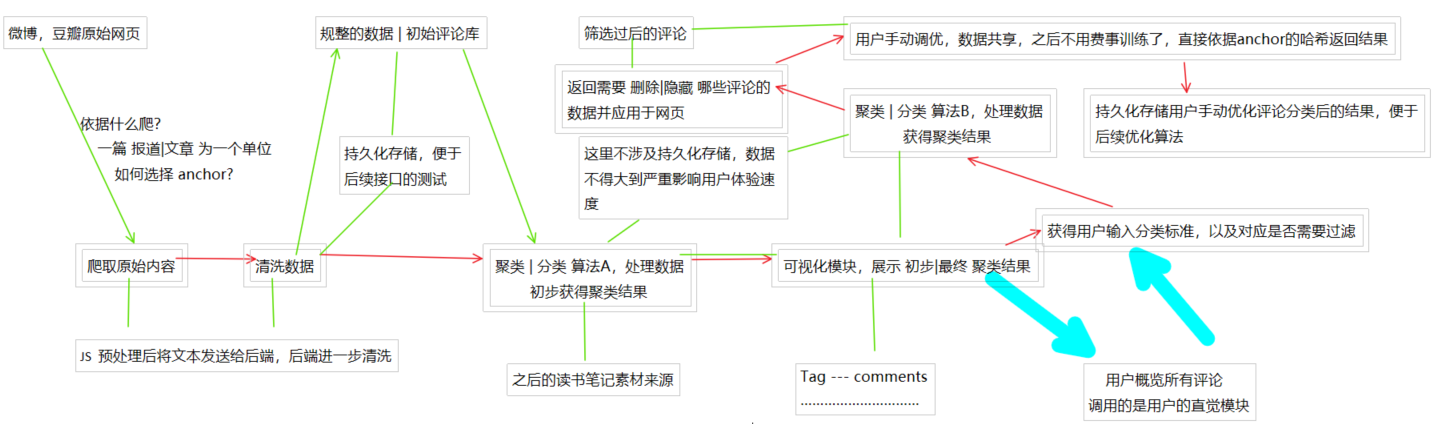
\includegraphics[scale=0.4]{art1.png}
\caption{系统设计}
\end{figure}

接下来的内容略写和业务逻辑相关的方面,详写和文本处理相关的方面。

\subsection{核心业务}
\subsubsection{爬取原始内容}

\subsubsection{清洗数据}

\subsubsection {聚类算法A}

\subsubsection{可视化模块}

\subsubsection{用户输入接口}

\subsubsection{聚类算法B}

\subsubsection{返回的数据}

\section {文本处理}
\subsection{基本概念}
把一个个文档的自然语言转换成数学信息,这样形成高维空间点之后再去计算点与点之间的距离,然后将这些距离比较近的聚成一个簇,这些簇的中心成为簇心.而我们做的就是保证簇内点的距离足够近,簇与簇的距离足够远。
\cite{zhihu1}

\subsection{文本聚类的过程}

\subsubsection{自动分词处理}
我们要把中文文章要进行分词,这一点中文文章和英文文章有一些区别,因为英文单词是单个构成的,也就不需要分词了,而我们中文是需要分词的,并且中文之间有一些词尽管大量出现,但是对于文章的分类结构起不到太大的意义,比如”的”,”了”,”么””应该”,这些词去计算他们既浪费空间又浪费时间,出于+1s的因素,我们也要节约时间啊,首先我们就加入一个停用词表,在进行分词的时候进行去掉。\cite{zhihu1}

\subsubsection{分词后将分词转换为词向量}
关于词向量我们有一些比较常用的模型,比如one-hotm,BOW词袋模型,连续词袋模型(CBOW)和Skip-Gram模型和Word2vec模型,在这次任务中我是用的是BOW词袋模型,在转换为词向量值我们要将其转换成tfidf矩阵,tfidf其实可以看作是提取的特征的一次加权,是根据一个单词在当前文章中出现的频率和该单词在所有语料中出现的频率评估一个单词的重要性,当一个单词在这篇文章中出现的次数很多的时候,这个词语更加重要;但如果它在所有文章中出现的次数都很多,那么它就显得不那么重要。\cite{zhihu1}

\subsubsection{选择聚类算法}
这里的算法大家常用的是K-means和DBSCAN,这两种算法用的最多,但是在高维空间里边K-means似乎并不是很好,究其原因是因为维度太高,簇与簇之间的距离太小了,如果直接去聚类,这一部分似乎效果不太好,这时候就需要用到主成分分析PCA,大致的思路是大致意思就是取这个高维向量中方差最大的方向经过一些数学变换将有用的部分保留,没用的部分舍弃,这种办法同样适合分类算法中寻找最大的特征。\cite{zhihu1}

我在前三篇读书笔记里已经分析了主流的无监督异常检测的聚类算法,这里不再赘述了。

\subsection{算法评测}
传统的角度:簇的距离,轮廓系数

实用的角度:主观评判

\subsubsection{参数调整}
根据不同的网站中爬下的大量的数据,经过人工的对算法分类结果的反馈与评定,分别设定对应的参数,使得之后的小数据(针对某篇文章、某个电影或某条微博)聚类算法(预处理阶段时候的分类)尽可能准确,方便后续的操作。

\section{文本相关过程使用到的工具}
\subsection{自动分词处理}
在信息检索中,为节省存储空间和提高搜索效率,在处理自然语言数据(或文本)之前或之后会自动过滤掉某些字或词,这些字或词即被称为Stop Words(停用词)。

这些停用词都是人工输入、非自动化生成的,生成后的停用词会形成一个停用词表。但是,并没有一个明确的停用词表能够适用于所有的工具,甚至有一些工具是明确地避免使用停用词来支持短语搜索的。

同义词(synonym)或者更学术性的称呼同义异形是世界上各种语言都存在的一种现象。它指的是表达的意义相同或相近,但是表达形式不同的词汇。

不仅词汇有同义现象,不同语法结构的句子也可以表示同一个意义。例如:

这本书非常有趣。
这是一本非常有趣的书。
同义词之间的差别主要有感情色彩、理性意义、语法特点、各地习惯的不同。

理性意义的差别又分别体现为范围、性状、程度等方面的不同。

感情色彩方面:“执着”与“固执”、“果断”与“武断”、“聪明”与“狡猾”

程度差别:“丰满”与“肥胖肥胖、“优秀”与“良好”、“少量”与“微量”
\subsubsection{jieba}
\subsection{将分词转换为词向量}
\subsubsection{doc2vec}
\subsubsection{word2vec}
\subsubsection{one-hotm}
\subsubsection{BOW}
\subsubsection{CBOW}
\subsubsection{Skip-Gram}
\subsection{可视化}
主要是要降维,之后不一定需要。
\subsubsection{PCA}
\subsubsection{TSNE}
\begin{figure}[ht]
\centering
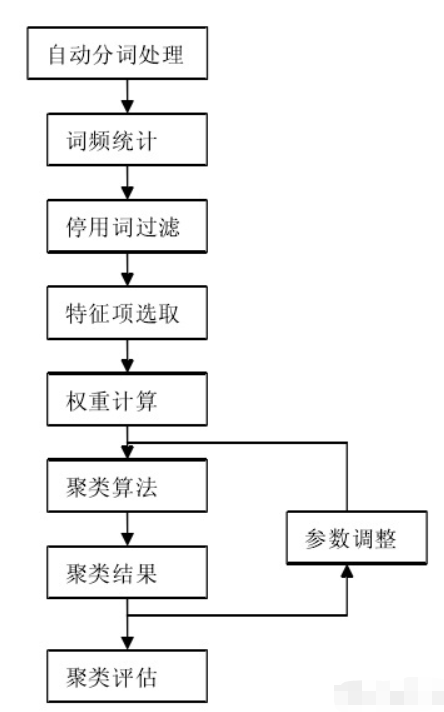
\includegraphics[scale=0.75]{NPLprocess.png}
\caption{文本聚类的过程}
\end{figure}

\section{各个工具的特点和原理}
\subsection{jieba}
中文分词的模型实现主要分类两大类:基于规则和基于统计。

1 基于规则
基于规则是指根据一个已有的词典,采用前向最大匹配、后向最大匹配、双向最大匹配等人工设定的规则来进行分词。

例如对于“上海自来水来自海上”这句话,使用前向最大匹配,即从前向后扫描,使分出来的词存在于词典中并且尽可能长,则可以得到“上海/自来水/来自/海上”。这类方法思想简单且易于实现,对数据量的要求也不高。

当然,分词所使用的规则可以设计得更复杂,从而使分词效果更理想。但是由于中文博大精深、语法千变万化,很难设计足够全面而通用的规则,并且具体的上下文语境、词语之间的搭配组合也都会影响到最终的分词结果,这些挑战都使得基于规则的分词模型愈发力不从心。

2 基于统计
基于统计是从大量人工标注语料中总结词的概率分布以及词之间的常用搭配,使用有监督学习训练分词模型。

对于“上海自来水来自海上”这句话,一个最简单的统计分词想法是,尝试所有可能的分词方案,因为任何两个字之间,要么需要切分,要么无需切分。

对于全部可能的分词方案,根据语料统计每种方案出现的概率,然后保留概率最大的一种。很显然,“上海/自来水/来自/海上”的出现概率比“上海自/来水/来自/海上”更高,因为“上海”和“自来水”在标注语料中出现的次数比“上海自”和“来水”更多。

3 jieba的原理
jieba分词结合了基于规则和基于统计两类方法。

首先基于前缀词典进行词图扫描,前缀词典是指词典中的词按照前缀包含的顺序排列,例如词典中出现了“上”,之后以“上”开头的词都会出现在这一块,例如“上海”,进而会出现“上海市”,从而形成一种层级包含结构。

如果将词看作节点,词和词之间的分词符看作边,那么一种分词方案则对应着从第一个字到最后一个字的一条分词路径。因此,基于前缀词典可以快速构建包含全部可能分词结果的有向无环图,这个图中包含多条分词路径,有向是指全部的路径都始于第一个字、止于最后一个字,无环是指节点之间不构成闭环。

基于标注语料,使用动态规划的方法可以找出最大概率路径,并将其作为最终的分词结果。

4 jieba三种分词模式以及其应用
jieba提供了三种分词模式:

精确模式:试图将句子最精确地切开,适合文本分析;
全模式:把句子中所有可以成词的词语都扫描出来, 速度非常快,但是不能解决歧义;
搜索引擎模式:在精确模式的基础上,对长词再次切分,提高召回率,适合用于搜索引擎分词。

\cite{xuqingtang}

\subsection{doc2vec}

\subsection{word2vec}

\subsection{one-hotm}

\subsection{BOW}

\subsection{CBOW}

\subsection{Skip-Gram}











\bibliography{cites.bib}
\bibliographystyle{ieeetr}

\end{document}